% !TeX spellcheck = en_GB
% !TeX program = xelatex
%
% LuxSleek-CV (Absolute Pixel-Perfect Alignment Fix)

\documentclass[11pt, a4paper]{article} 

\usepackage{fontspec}
\usepackage[british]{babel}  
\usepackage[left = 0mm, right = 0mm, top = 0mm, bottom = 0mm]{geometry}
\usepackage[stretch = 25, shrink = 25]{microtype}  
\usepackage{graphicx}        
\usepackage{xcolor}          
\usepackage{marvosym}        
\usepackage{fontawesome5}    

\usepackage{enumitem}        
\setlist{parsep = 0pt, topsep = 0pt, partopsep = 0pt, itemsep = 1pt, leftmargin = 4.5mm}

\usepackage{FiraSans}        
\renewcommand{\familydefault}{\sfdefault}

\definecolor{cvblue}{HTML}{000624}
\definecolor{linkblue}{HTML}{0044cc}

%%%%%%% USER COMMAND DEFINITIONS %%%%%%%%%%%%%%%%%%%%%%%%%%%
\newcommand{\dates}[1]{\hfill\mbox{\textbf{#1}}} 
% Ép khoảng cách xuống 0.1ex (Khoảng thở siêu mỏng, an toàn tuyệt đối)
\newcommand{\is}{\par\vspace*{0.1ex}} 
\newcommand{\smaller}[1]{{\small$\diamond$\ #1}}
% Gọt dũa tối đa margin các thẻ Headings
\newcommand{\headleft}[1]{\vspace*{0.8ex}\textsc{\textbf{#1}}\par%
    \vspace*{-1.2ex}\hrulefill\par\vspace*{0.2ex}}
% ĐÃ THÊM \textbf{#1} VÀO ĐÂY ĐỂ IN ĐẬM TIÊU ĐỀ CỘT PHẢI
\newcommand{\headright}[1]{\vspace*{0.4ex}\textsc{\Large\color{cvblue}\textbf{#1}}\par%
     \vspace*{-1.2ex}{\color{cvblue}\hrulefill}\par\vspace*{0.2ex}}
%%%%%%%%%%%%%%%%%%%%%%%%%%%%%%%%%%%%%%%%%%%%%%%%%%%%%%%%%%%%

\usepackage[colorlinks = true, urlcolor = linkblue, linkcolor = linkblue]{hyperref}

\begin{document}

% Mở rộng trang ảo 25mm - Giới hạn tối đa an toàn khi in ấn
\enlargethispage{25mm}

\setlength{\topskip}{0pt}
\setlength{\parindent}{0pt}
\setlength{\parskip}{0pt}
\setlength{\fboxsep}{0pt}
\pagestyle{empty}
\raggedbottom

\begin{minipage}[t]{0.33\textwidth} %% LEFT COLUMN
\vspace{0pt}\vspace{-\baselineskip} 
\colorbox{cvblue}{\begin{minipage}[t][5mm][t]{\textwidth}\null\hfill\null\end{minipage}}

\vspace{-.2ex} 
\colorbox{cvblue!90}{\color{white}  
\kern0.08\textwidth\relax
% Khối xanh dài 310mm để tràn đáy hoàn hảo
\begin{minipage}[t][310mm][t]{0.84\textwidth}
\raggedright
\vspace*{1.5ex}

\Large \textbf{\textsc{Huỳnh Quốc Huy}} \normalsize \\
\small \textbf{{Junior Full-Stack Developer}} \normalsize

\vspace*{1ex}
\null\hfill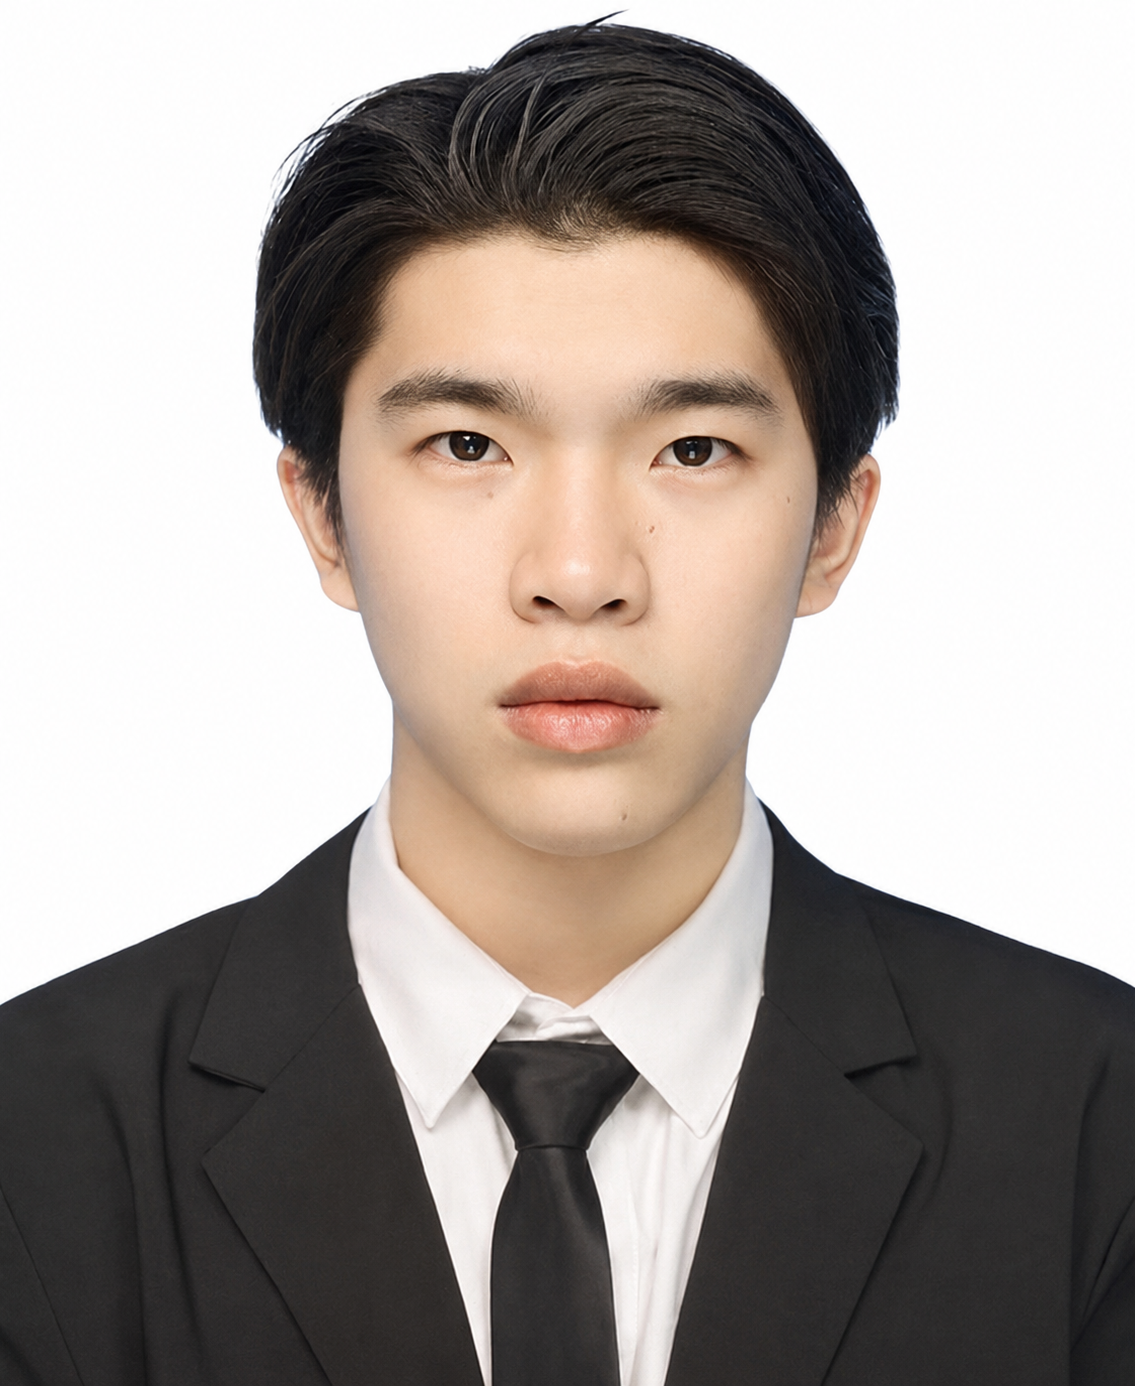
\includegraphics[width=0.75\textwidth]{huynhquochuy.jpg}\hfill\null
\vspace*{1ex}

\headleft{Personal Information}
\small 
\faPhone\ +84-924-202-149 \\
\faMapMarker\ An Giang, Vietnam \\
\faEnvelope\ \href{mailto:huykyunh.k@gmail.com}{\color{white}{huykyunh.k@gmail.com}} \\

\faGlobe\ Languages: \\ 
\smaller{Vietnamese~(Native)} \\
\smaller{English~(B2 Level)} \\ 
\smaller{Chinese~(Basic)}

\headleft{Social Media}
\small 
\faGithub\ \href{https://github.com/hkhuang07}{\color{white}{github.com/hkhuang07}}\\
\faLinkedin\ \href{https://www.linkedin.com/in/hkhuang07/}{\color{white}{linkedin.com/in/hkhuang07}} \\
\normalsize

\headleft{Education}
\small
\smaller{\textbf{B.S. in IT} \textbf{An Giang University} \dates{(2026 Expected)}} \\
\smaller{\textbf{GPA:} 3.30/4.0 (Scale 10: 8.09) } \\
\smaller{\textbf{Core Coursework:} Oracle DB, Blockchain, Cloud Computing, Cyber Security, IoT, Java Android, OSS...} \\
\smaller{\textbf{CS50:} Introduction to Computer Science at edX. \textbf{(June-July 2024)} }
\normalsize 

\headleft{Certificates \& Awards}
\small
\faIcon{certificate} \textsf{VSTEP English Proficiency} \\ \textsf{Certificate} \textbf{(B2 Level)}\\
\faIcon{award} {Awards:} \\
\smaller{\textbf{ATV Tiep Buoc Den Truong}} Scholarship \\
\smaller{\textbf{Tiep Suc}} Scholarship

\headleft{Soft Skills}
\small
\smaller{\textbf{Problem-solving:} Aptitude for Root Cause. Capable of diagnosing low-level system anomalies and architecting resilient structural fixes rather than surface-level patches.}
\is
\smaller{\textbf{Teamwork \& Collaboration:} respect teamwork , adhering to GitFlow in collaborative projects.}
\is
\smaller{\(\textbf{Continuous\ Learning:}\) Proactively mastering modern technologies and engineering paradigms via documentation and AI.}\is
\is
\smaller{\textbf{Communication \& Presentation:} Friendly communication style, presenting issues clearly, coherently, and confidently.}
\normalsize

\end{minipage}
\kern0.08\textwidth\relax
}
\end{minipage}% 
\hskip2em%% RIGHT COLUMN
\begin{minipage}[t]{0.59\textwidth}
\vspace{0pt} 
\raggedright
\setlength{\parskip}{0pt}
% Tăng khoảng cách title Career Objective với rìa top
\vspace*{3mm}

\headright{Career Objective}
\is
\small
Progressive and highly motivated Full-Stack Developer leveraging technical foundations, system architecture, a programming mindset, and practical experience to build and contribute to projects. Through this, I aim to optimize systems for high scalability, delivering maximum business value to the enterprise. Possessing a spirit of continuous learning, accountability, dedication, and professional integrity. Furthermore, I strategically integrate AI to accelerate development and optimize processing, driven by a long-term vision of advancing to Senior Developer and Software Architect roles.

\headright{Work Experience}
\is
\textbf{SoftZ Corporation} \hfill \dates{02/2026 -- 04/2026} \\
\textit{Full-Stack Intern (Internship Score: 9.5/10)}
\is
\smaller{\textbf{System Analysis \& Documentation:} Assimilated core system analysis blueprints and authored extended documentation including integration workflows, API documentation, and UI designs for the EInvoiceHub middleware.}
\is
\smaller{\textbf{Backend Architecture:} Developed the EInvoiceHub backend system using Spring Boot, leveraging Adapter/Strategy patterns to unify JSON/XML integrations across multiple TVAN providers (BKAV, MobiFone).}
\is
\smaller{\textbf{Full-Stack Automation:} Engineered dynamic Angular dashboards for invoice management. Implemented Spring Batch cron jobs for automated bulk digital signing and real-time status synchronization with tax authorities, eliminating manual workload.}

\headright{Key Projects}
\is
% 1. DiginvoiceStation
\textbf{Diginvoice Station} | \textit{Spring Boot, Java 21 \& GitOps} \hfill \dates{01/2026 -- 05/2026} \\
\smaller{Resolved network I/O bottlenecks utilizing Java 21 Virtual Threads, enabling the concurrent processing of external API connections without exhausting OS threads. Eliminated Out-Of-Memory (OOM) risks during automated bulk digital signing by leveraging the Chunk-Based and Fault-Tolerant mechanisms of Spring Batch. Eradicated manual deployment errors by engineering a fully automated GitOps CI/CD pipeline (ArgoCD, Terraform, K3d), establishing Cloud-Ready operational standards.}
\is
% 2. HK-07 Hugo Sanitas Robot
\textbf{Hugo Sanitas HK-07 Robot} | \textit{Python, CV, SLM \& ROS 2} \hfill \dates{05/2026 -- Present} \\
\smaller{Optimized a healthcare companion stack (ROS 2, FastAPI, Spring Boot) under severe hardware constraints, budgeting total memory usage to <615MB RAM. Engineered an ultra-low latency (<5ms) deterministic MQTT pipeline for high-priority safety reflexes and motion inhibition. Implemented dual-factor fall detection and local edge fallback capabilities leveraging Ollama and llama-cpp (GGUF SLMs) for offline empathetic companion dialogue.}
\is
% 3. Sales Management System
\textbf{Electronics Store} | \textit{Client-Server, C\# .NET EF Core} \hfill \dates{06/2025 -- 07/2025} \\
\smaller{Identified and resolved the structural limitations and security vulnerabilities of legacy academic models by refactoring a monolithic codebase into a strict, distributed 4-Layer architecture (Client $\rightarrow$ Server $\rightarrow$ Business Logic $\rightarrow$ Data Access). Guaranteed atomic transaction integrity and eliminated raw-query risks by integrating Entity Framework Core with the Unit of Work pattern. Prevented TCP stream fragmentation (split/combined messages) by engineering a custom length-prefixed socket framing protocol, ensuring highly reliable multi-threaded JSON payload transmissions.}

\headright{Technical Skills \& Core Competencies}
\is
\smaller{\textbf{Backend \& Integration (Java Spring Boot):} Capable of applying Design Patterns (Adapter/Strategy) to build extensible API integrations that share a unified database schema. Experienced in automating repetitive manual workflows and ensuring data synchronization using Spring Batch cron jobs.}
\is
\smaller{\textbf{Architecture \& ORM (C\# .NET):} Able to refactor unstructured academic code into clean, multi-tier architectures (4-Layer Client-Server). Skilled in securing queries and managing data integrity using Entity Framework Core and the Unit of Work pattern over TCP sockets.}
\is
\smaller{\textbf{DevOps \& CI/CD (Docker, GitOps):} Practical understanding of continuous delivery. Able to transition from manual Windows setups to automated, containerized Linux (WSL) pipelines using GitHub Actions, ArgoCD, and K3d to simulate cloud-ready environments.}
\is
\smaller{\(\textbf{Full-Stack\ Adaptability:}\) Understanding of web fundamentals (Vue.js, Node.js, PHP) and databases (SQL Server, MySQL). Effectively utilizes AI agents for document research and analysis, process optimization, system integration, scalability and stability enhancement, and troubleshoot errors.}

\end{minipage}

\end{document}